\documentclass[a4paper,12pt, oneside]{book}

%\usepackage{fullpage}
\usepackage[italian]{babel}
\usepackage[utf8]{inputenc}
\usepackage{amssymb}
\usepackage{amsthm}
\usepackage{graphics}
\usepackage{amsfonts}
\usepackage{amsmath}
\usepackage{amstext}
\usepackage{engrec}
\usepackage{rotating}
\usepackage[safe,extra]{tipa}
\usepackage{showkeys}
\usepackage{multirow}
\usepackage{hyperref}
\usepackage{microtype}
\usepackage{enumerate}
\usepackage{braket}
\usepackage{marginnote}
\usepackage{pgfplots}
\usepackage{cancel}
\usepackage{polynom}
\usepackage{booktabs}
\usepackage{enumitem}
\usepackage{framed}
\usepackage{pdfpages}
\usepackage{pgfplots}
\usepackage{fancyhdr}
\pagestyle{fancy}
\fancyhead[LE,RO]{\slshape \rightmark}
\fancyhead[LO,RE]{\slshape \leftmark}
\fancyfoot[C]{\thepage}



\title{Reti e sistemi}
\author{UniShare\\\\Davide Cozzi\\\href{https://t.me/dlcgold}{@dlcgold}\\\\Gabriele De Rosa\\\href{https://t.me/derogab}{@derogab} \\\\Federica Di Lauro\\\href{https://t.me/f_dila}{@f\textunderscore dila}}
\date{}

\pgfplotsset{compat=1.13}
\begin{document}
\maketitle

\definecolor{shadecolor}{gray}{0.80}

\newtheorem{teorema}{Teorema}
\newtheorem{definizione}{Definizione}
\newtheorem{esempio}{Esempio}
\newtheorem{corollario}{Corollario}
\newtheorem{lemma}{Lemma}
\newtheorem{osservazione}{Osservazione}
\newtheorem{nota}{Nota}
\tableofcontents
\renewcommand{\chaptermark}[1]{%
\markboth{\chaptername
\ \thechapter.\ #1}{}}
\renewcommand{\sectionmark}[1]{\markright{\thesection.\ #1}}

\chapter{Introduzione}
\textbf{Questi appunti sono presi a lezione. Per quanto sia stata fatta una revisione è altamente probabile (praticamente certo) che possano contenere errori, sia di stampa che di vero e proprio contenuto. Per eventuali proposte di correzione effettuare una pull request. Link: } \url{https://github.com/dlcgold/Appunti}.\\
\textbf{Grazie mille e buono studio!}

\section{Reti}
%11
Una rete è visualizzabile come un grafo, con punti terminali uniti in maniera efficiente. Questi punti terminali sono chiamati \textbf{nodi}. Le reti di cui parliamo sono le moderne reti \textit{TCP/IP}, con regole chiamate \textit{protocolli}. Internet è una rete che connette miliardi di punti terminali, con regole \textit{end to end} comuni. Internet significa infatti \textit{interconnected networks}, \textit{reti interconnesse}. Internet è costituita da tante componenti gestite autonomamente (chiamate \textbf{AS}, \textit{autonomus system}) collegate tra loro. Ci sono regole per lo scambio di informazioni tra i vari AS. un po' di terminologia:
\begin{itemize}
\item gli \textbf{host} sono i vari punti terminali, come pc, server... fino al \textit{trasporto} i protocolli sono uguali
\item i \textbf{router} sono i vari nodi nella rete. Essi sono contenuti negli AS e sono collegati tra loro in un AS e collegati a router di altri AS
\item il collegamento tra host e il primo router si chiama \textbf{Accesso/link}, che può essere un filo o una particolare rete che permette a tanti terminali di collegarsi al router (fatta con fili, è la tecnologia \textit{ethernet}, o wireless, col filo che si ferma ad un trasmettitore e tanti oggetti che parlano via radio, è la tecnologia \textit{wifi}, protocollo 801.11 o 811.3)
\item il \textbf{forwarding} è l'azione del nodo che trasferisce un dato da un punto d'ingresso ad uno di uscita 
\item ciò che stabilisce la strada migliore è un insieme di algoritmi che realizzano il \textbf{routing}
\item un elemento di informazione è detto \textbf{pacchetto}, ovvero un blocco di dati (\textbf{payload}) con un'intestazione (\textbf{header}), che contiene le informazioni per gestire il protocollo, come l'\textbf{indirizzo} di destinazione , o ancora meglio gli \textbf{indirizzi}di destinazione e sorgente, come un \textbf{contatore} che tiene conto del numero di pacchetti contenuti per controllare il completo trasferimento dei dati. Alcuni protocolli, come l'ethernet, hanno anche un \textbf{trailer}.
\item per trasferire file di grandi dimensione, per evitare perdite, intasamento dei nodi etc..., si effettua uno spezzamento e l'inserimento in una sequenza di pacchetti. Questa operazione è la \textbf{pacchettizzazione}
\item i protocolli sono in realtà \textbf{protocolli stratificati}. Si suppongano due nodi $X$ e $Y$ e un trasferimento di pacchetti tra loro e dal secondo viene poi mandato in altre due direzioni $A$ e $B$. Appena il pacchetto arriva a $Y$ si deve capire dove inizia e finisce il pacchetto, capire se tutti i bit sono giusti, e se non lo sono ritrasmettere il pacchetto, si deve capire com'è fatto, capire il destinatario per decidere quale uscita usare ($A$ o $B$). Un pacchetto contiene e varie informazioni, a strati, si, per esempio, ha un protocollo P1 per capire se è corretto. Poi dentro il payload si avrà un altro protocollo P2 per i dati di routering e forwarding. 
\item un insieme di protocolli uno sopra l'altro si chiama di \textbf{stack internet} e si hanno i protocolli di \textbf{livello fisico}, quelli più elementari, con regole di logica ed elettronica (come è fatto un bit etc...), il \textbf{livello di datalink}, con protocolli più alti (indicazioni di inizio e fine di un pacchetto, correttezza, destinazione etc...), sopra ancora si ha il \textbf{livello IP/rete} (che si occupa di routing), sopra si ha il \textbf{livello di trasporto} (come TCP) e sopra ancora il \textbf{livello applicativo} (con operazioni più complesse e specifiche). Quest'ultimo livello è fatto da programmi su un calcolatore, i \textbf{processi/threads} e in questo livello il sistema operativo fornisce le interfacce di comunicazione, i \textbf{socket} (a cui non interessano i trasporti intrinsechi della rete). Ogni protocollo toglie lavoro a quello sopra, ovvero \textbf{offre un servizio}. Dal fisico al datalink si ha un servizio di codifica e trasmissione, dsl datalink al l'ip è di formattazione dei blocchi e correttezza, da ip a trasporto è di instradamento e consegna, e da trasporto a applicazione è di comunicazione trasparente end-to-end con molte funzioni. Nessuno strato fornisce un servizio a tutti gli altri direttamente. Si spezza così il problema in più parti, facilitando l'implementazione di funzioni e il loro test. 
\end{itemize}
Parliamo ora di prestazioni. Una rete va bene o male in base a:
\begin{itemize}
\item \textbf{ritardi}, spesso del software non è usabile se la rete ritarda troppo
\item \textbf{throughput}, ovvero la quantità di dati che può passare
\end{itemize}
Iniziamo dai ritardi. Immaginiamo un collegamento tra due host con due nodi in mezzo. Trasmetto un pacchetto di lunghezza $l$. Chiamo $r$ la velocità del link, in $\frac{bit}{s}$. Il tempo di trasferimento sarà di $t=\frac{l}{r}$, detto anche \textbf{ritardo di trasmissione}. Ovviamente il Primo bit arriverà prima e l'ultimo dopo. Chiamo $s$ la velocità della luce nel mezzo. Tra un  host e un nodo ci sarà un tempo di propagazione $\frac{d}{s}$, con $d$ distanza fisica tra i terminali, dato dalla velocità della luce. Si ha poi il tempo di processing (di pochi millisecondi, durante il quale vengono eseguite le operazioni base per identificare destinazione etc...) $t_{proc}$ e il tempo di queuing (nel quale si decide con che ordine far uscire i pacchetti verso una certa destinazioni, mettendoli in una coda; anche questo è un tempo minimo) $t_q$; $t_{proc}+t_q$ è un ritardo interno al nodo ed è minimo. Il ritardo di trasmissione è quasi nullo tra due nodi. Ma il tempo di accesso dipende da fibra ottica etc... ed è la parte che fa maggiormente la differenza. Il througput sarà comunque pari al punto più ristretto della banda.
Quanto detto si può vedere nella seguente immagine:
\begin{center}
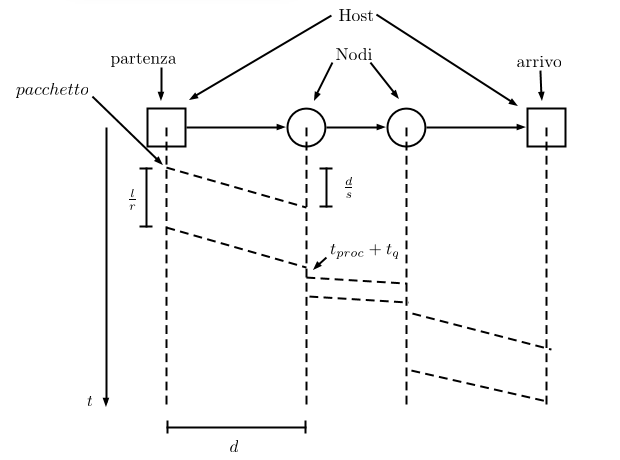
\includegraphics[scale=0.5]{img/reti.png}
\end{center}
\section{Sistemi Operativi}
Un sistema operativo gestisce le risorse virtuali, ormai non gestisce più direttamente l'hardware. Inoltre ora si hanno quasi solo sistemi con cpu multicore (o anche multiprocessing, ovvero con più cpu a più core). Gestisce anche la memoria, sia RAM che memoria di massa (HDD e SSD). Attualmente molti sistemi sono eterogenei (con più GPU etc...). Alcune CPU hanno core a diverse prestazioni e consumi e questa cosa va gestita dal sistema operativo. Ormai si ha inoltre molta virtualizzazione, con più macchine virtuali su una stessa macchina. Questo comporta maggior versatilità, meno rischi, comodità nel cloud, comodità di trasferimento di macchine virtuali etc.... Questo mondo è continuamente in evoluzione. Un sistema operativo quindi è un ambiente software che consente a più utenti di lavorare correttamente gestendo le risorse. Quindi:
\begin{itemize}
\item l'os deve coordinare le varie attività, mediante sincronizzazione etc.... Ogni os fornisce delle \textit{primitive di sincronizzazione}
\item l'os deve occuparsi dello \textit{scheduling delle risorse}, ovvero di gestione delle risorse. Ad ogni programma  si lasciano tot risorse e non per sempre
\item l'os gestisce le \textit{interfacce di programmazione}, permettendo maggior astrazione al developer. Riducendo ancora i rischi. I programmi lavoreranno in un ambiente "protetto" e scriverà dati in un altro processo solo in maniera estremamente controllata. 
\item l'os impedisce l'accesso diretto dei software ai driver fisici. Si occupa anche di sicurezza, impedendo ad un software di distruggere un altro processo. Lavora anche in termini di \textit{Cyber Security}. 
\item l'os si occupa anche di performance, gestendo le risorse in maniera ottimizzata. Si ha quindi la gestione di \textit{priorità} e di \textit{timer}
\item l'os gestisce infine, in maniera trasparente e automatica, le risorse. Per esempio alimentazione, ventole etc.... 
\end{itemize}
Esiste anche un altro punto di vista. L'os fornisce API e System Call. Da questo punto di vista l'os è un fornitore di servizi, interfacce (grafiche o testuali). Un software viene gestito in maniera diverso da un os per PC/Workstation (dove si ha multiprogrammazione, gestione della sicurezza, una GUI ma non si ha gestione di molte applicazioni identiche) e uno da server (non si ha una GUI ma si ha un'ottima efficienza di throughput e ottima gestione di software identico e delle risorse) e uno per smartphone (dove si ha la gestione del touchscreeen, la presenza di molti sensori etc...). Si hanno poi i sistemi embedded con la gestione \textit{real time}. \\
Un paio di concetti:
\begin{itemize}
\item un \textit{processo} è un codice in esecuzione che vive in un proprio spazio di memoria virtuale (che è la memoria fisica vista in maniera astratta). Un \textit{thread} è un flusso di esecuzione indipendente, ma tanti thread possono condividere lo stesso spazio di memoria virtuale
\item esistono più modalità di esecuzione:
\begin{itemize}
\item \textit{user mode} con limiti di accesso alle risorse fisiche. Si ha una "zona" più sicura. Si può accedere alle risorse di sistema con le system call (che interfacciano la user mode alla kernel mode), codice dell'os che si presume funzionante. La gestione delle eccezioni è una syscall. Con le syscall si accede alle APi del sistema operativo.  
\item \textit{kernel mode} con accesso completo alle risorse del sistema, scrivere codice a livello kernel è molto delicato. Qui si ha il codice per lo scheduling, gestione della memoria, gestione della rete etc...
\item nel caso di macchina virtuale si hanno tre livelli:
\begin{itemize}
\item Os Host
\item Os guest
\item livello applicativo
\end{itemize}
\end{itemize}
\end{itemize}
Ci sono poche possibilità per strutturare un sistema operativo. Molti os hanno un kernel \textit{monolitico}, con un kernel unico (un solo blocco di codice), per esempio Linux. Questa è una soluzione efficiente perché la comunicazione tra le componenti è semplice e veloce. Un'altra opzione è un os stratificato, ma è talmente poco ottimizzato (si ha un overhead, un insieme di istruzioni inutili, estremo) che non viene usata come soluzione, anche se il sistema dei driver di Windows è stratificato. l'altro modello è quello del \textit{micro-kernel}, che consiste in poche funzionalità essenziali nel kernel e tutto il resto viene spostato in modalità utente (anche cose come il file system). Questa soluzione è efficiente e sicura, e parzialmente viene usata da Apple in MacOS. \\
Ecco una lista delle principali famiglie di syscall Unix:
\begin{itemize}
\item controllo dei processi:
\begin{itemize}
\item creazione e terminazione dei processi
\item sincronizzazione dei processi (con le primitive \textit{wait} e \textit{signal})
\item gestione di attributi e priorità
\end{itemize}
\item comunicazione dei processi:
\begin{itemize}
\item memoria comune
\item messaggistica
\item connessioni (creazione di flussi di byte tra due processi, \textit{bytestream})
\end{itemize}
\item file management:
\begin{itemize}
\item creazione e cancellazione di un file
\item apertura e chiusura di un file
\item operazioni di \textit{read, write, append, etc...}
\item gestione di attributi e permessi di accesso
\end{itemize}
\item device management:
\begin{itemize}
\item installazione e disinstallazione di un device, con riconoscimento del device tramite i driver
\item apertura, chiusura, scrittura, gestione attributi etc... Queste cose sono simili al file management infatti alcuni os (basati su Unix, per esempio) vedono i device come file, ad un certo livello di astrazione.
\end{itemize}
\item gestione delle informazioni statistiche e di sistema:
\begin{itemize}
\item calcolo dell'uso delle risorse etc...
\item numero processi attivi e controllo del loro uso di risorse
\end{itemize}
\end{itemize}
\chapter{Reti}
\end{document}